\documentclass[10pt,aspectratio=169]{beamer}

% ============================================
% PACKAGES
% ============================================
\usepackage[utf8]{inputenc}
\usepackage[T1]{fontenc}
\usepackage[french,provide=*]{babel}
\usepackage{amsmath,amssymb,amsthm}
\usepackage{mathtools}
\usepackage{bm}
\usepackage{graphicx}
\usepackage{booktabs}
\usepackage{tikz}
\usetikzlibrary{arrows.meta,positioning,shapes,calc,decorations.pathreplacing}
\usepackage{hyperref}

% ============================================
% THEME ET COULEURS
% ============================================
\usetheme{Madrid}
\usecolortheme{whale}

\definecolor{darkblue}{RGB}{0,51,102}
\definecolor{lightblue}{RGB}{230,240,250}
\definecolor{darkgreen}{RGB}{0,102,51}
\definecolor{darkred}{RGB}{153,0,0}
\definecolor{orange}{RGB}{255,128,0}

\setbeamercolor{structure}{fg=darkblue}
\setbeamercolor{block title}{bg=darkblue,fg=white}
\setbeamercolor{block body}{bg=lightblue,fg=black}
\setbeamercolor{block title example}{bg=darkgreen,fg=white}
\setbeamercolor{block body example}{bg=green!10,fg=black}
\setbeamercolor{block title alerted}{bg=darkred,fg=white}
\setbeamercolor{block body alerted}{bg=red!10,fg=black}

% ============================================
% ENVIRONNEMENTS THÉORÈMES
% ============================================
\theoremstyle{definition}
\newtheorem{definitionfr}{Définition}
\newtheorem{exemplefr}{Exemple}
\newtheorem{remarquefr}{Remarque}
\newtheorem{propositionfr}{Proposition}
\newtheorem{theoremefr}{Théorème}
\newtheorem{corollairefr}{Corollaire}
\newtheorem{lemmefr}{Lemme}
\newtheorem{proprietefr}{Propriété}

% ============================================
% COMMANDES PERSONNALISÉES
% ============================================
\newcommand{\E}{\mathbb{E}}
\newcommand{\Var}{\mathbb{V}}
\newcommand{\Cov}{\mathrm{Cov}}
\newcommand{\Prob}{\mathbb{P}}
\newcommand{\R}{\mathbb{R}}
\newcommand{\N}{\mathbb{N}}
\newcommand{\indep}{\perp\!\!\!\perp}
\newcommand{\plim}{\overset{p}{\longrightarrow}}
\newcommand{\dlim}{\overset{d}{\longrightarrow}}
\newcommand{\aslim}{\overset{a.s.}{\longrightarrow}}
\DeclareMathOperator*{\argmax}{arg\,max}
\DeclareMathOperator*{\argmin}{arg\,min}

% ============================================
% INFORMATIONS DU DOCUMENT
% ============================================
\title[Économétrie des Variables Qualitatives]{Économétrie des Variables Qualitatives}
\subtitle{Introduction}
\date{Janvier, 2026}

\begin{document}

% ============================================
% PAGE DE TITRE
% ============================================
\begin{frame}
    \titlepage
\end{frame}

% ============================================
% PLAN
% ============================================
\begin{frame}{Plan du cours}
    \begin{columns}[T]
        \begin{column}{0.48\textwidth}
            \begin{block}{\textcolor{darkblue}{\textbf{PARTIE I}} — Variables explicatives}
                \small
                Variables qualitatives \textbf{à droite} de l'équation
                \vspace{0.2cm}
                \begin{itemize}
                    \item Modèle sans terme constant
                    \item Modèle avec terme constant
                    \item Modèle avec variables explicatives
                    \item Modèle avec produits croisés
                \end{itemize}
            \end{block}
        \end{column}
        \begin{column}{0.48\textwidth}
            \begin{block}{\textcolor{darkgreen}{\textbf{PARTIE II}} — Variables expliquées}
                \small
                Variables qualitatives \textbf{à gauche} de l'équation
                \vspace{0.2cm}
                \begin{itemize}
                    \item Variables dichotomiques
                    \item Variables polytomiques ordonnées
                    \item Variables de comptage
                    \item Variables censurées/tronquées
                \end{itemize}
            \end{block}
        \end{column}
    \end{columns}
    
    \vspace{0.5cm}
    
    \begin{center}
        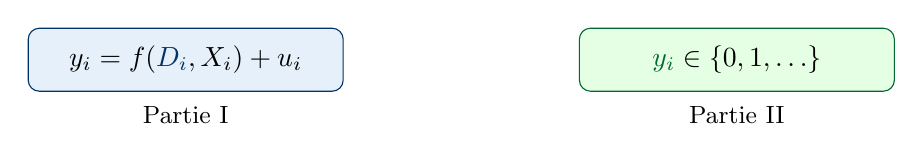
\begin{tikzpicture}
            \node[rectangle, draw=darkblue, fill=lightblue, rounded corners, minimum width=4cm, minimum height=0.8cm] (exp) at (0,0) {$y_i = f(\textcolor{darkblue}{D_i}, X_i) + u_i$};
            \node[rectangle, draw=darkgreen, fill=green!10, rounded corners, minimum width=4cm, minimum height=0.8cm] (exq) at (7,0) {$\textcolor{darkgreen}{y_i} \in \{0,1,\ldots\}$};
            \node at (0,-0.7) {\small Partie I};
            \node at (7,-0.7) {\small Partie II};
        \end{tikzpicture}
    \end{center}
\end{frame}

% ============================================
% PARTIE I : VARIABLES QUALITATIVES EXPLICATIVES
% ============================================


\setbeamercolor{background canvas}{bg=darkblue}
\setbeamercolor{normal text}{fg=white}
\usebeamercolor[fg]{normal text}
\begin{frame}[plain]
    \vfill
    \begin{center}
        {\Huge\bfseries PARTIE I}
        
        \vspace{1cm}
        
        {\LARGE Les variables qualitatives}
        
        \vspace{0.3cm}
        
        {\LARGE\bfseries EXPLICATIVES}
        
        \vspace{1.5cm}
        
        {\large Variables qualitatives à droite de l'équation}
        
        \vspace{0.3cm}
        
        {\large $y_i = f(\textcolor{orange}{D_i}, X_i) + u_i$}
    \end{center}
    \vfill
\end{frame}


\section{Les variables qualitatives explicatives}

\begin{frame}{Introduction}
    \begin{block}{Contexte}
        Les variables qualitatives explicatives sont omniprésentes en économie appliquée :
        \begin{itemize}
            \item Économie du travail : genre, niveau de diplôme, catégorie socio-professionnelle
            \item Économie de l'innovation : secteur d'activité, région, taille d'entreprise
            \item Économie industrielle : appartenance à un groupe, type de marché
        \end{itemize}
    \end{block}
    
    \vspace{0.3cm}
    
    \begin{block}{Objectif}
        Comprendre l'interprétation des coefficients des variables qualitatives dans le modèle linéaire et ses extensions.
    \end{block}
\end{frame}

\begin{frame}{Deux utilisations principales}
    \begin{enumerate}
        \item \textbf{Effets fixes catégoriels} : indicatrices d'appartenance à un groupe
        \begin{itemize}
            \item Les coefficients s'interprètent comme des \alert{écarts moyens} par rapport à une modalité de référence
            \item Ils ne représentent plus des dérivées (qui n'existent pas)
        \end{itemize}
        
        \vspace{0.4cm}
        
        \item \textbf{Approximation de fonctions non linéaires} : 
        \begin{itemize}
            \item Découpage d'une variable continue en intervalles
            \item Estimation d'une relation non paramétrique par morceaux
        \end{itemize}
    \end{enumerate}
\end{frame}

% --------------------------------------------
\subsection{Modèle sans terme constant}

\begin{frame}{Modèle sans terme constant : Formalisation}
    \begin{definitionfr}[Variable qualitative polytomique]
        Soit une variable qualitative à $p$ modalités. Pour un échantillon de $N$ individus, on définit les ensembles d'indices :
        \[
        G_j = \{i : \text{individu } i \text{ appartient au groupe } j\}, \quad j = 1, \ldots, p
        \]
        avec $\bigcup_{j=1}^{p} G_j = \{1, \ldots, N\}$ (partition).
    \end{definitionfr}
    
    \vspace{0.3cm}
    
    \begin{definitionfr}[Indicatrices]
        Les variables dichotomiques associées sont définies par :
        \[
        D_{ji} = \begin{cases}
            1 & \text{si } i \in G_j \\
            0 & \text{si } i \notin G_j
        \end{cases}, \quad i = 1, \ldots, N
        \]
    \end{definitionfr}
\end{frame}

\begin{frame}{Propriétés fondamentales des indicatrices}
    \begin{proprietefr}
        Les variables indicatrices vérifient les propriétés suivantes :
        \begin{enumerate}
            \item \textbf{Idempotence} : $D_{ji}^2 = D_{ji}$ \quad (car $0^2 = 0$ et $1^2 = 1$)
            
            \vspace{0.2cm}
            
            \item \textbf{Exclusivité mutuelle} : $D_{ji} \cdot D_{ki} = 0$ pour tout $j \neq k$
            
            \vspace{0.2cm}
            
            \item \textbf{Effectif du groupe} : $\displaystyle\sum_{i=1}^{N} D_{ji} = N_j$
            
            \vspace{0.2cm}
            
            \item \textbf{Fréquence du groupe} : $\displaystyle\frac{1}{N} \sum_{i=1}^{N} D_{ji} = \frac{N_j}{N}$
        \end{enumerate}
    \end{proprietefr}
    
    \begin{remarquefr}
        La propriété 4 montre que pour les indicatrices, la moyenne arithmétique calcule des pourcentages.
    \end{remarquefr}
\end{frame}

\begin{frame}{Le modèle linéaire avec indicatrices}
    \begin{block}{Spécification}
        Le modèle linéaire s'écrit :
        \[
        y_i = \sum_{j=1}^{p} b_j D_{ji} + u_i, \quad i = 1, \ldots, N
        \]
        avec les hypothèses classiques sur les perturbations :
        \[
        \E(u_i) = 0, \quad \E(u_i^2) = \sigma_u^2, \quad \E(u_i u_j) = 0 \text{ pour } i \neq j
        \]
    \end{block}
    
    \vspace{0.3cm}
    
    \begin{propositionfr}[Interprétation des coefficients]
        L'espérance conditionnelle dans le groupe $j$ est :
        \[
        \E(y_i \mid D) = b_j \quad \text{si } i \in G_j
        \]
        Les coefficients représentent donc les \alert{moyennes conditionnelles par groupe}.
    \end{propositionfr}
\end{frame}

\begin{frame}{Différence entre groupes}
    \begin{corollairefr}
        La différence entre deux coefficients s'interprète comme la différence des espérances conditionnelles :
        \[
        b_j - b_k = \E(y_i \mid i \in G_j) - \E(y_i \mid i \in G_k)
        \]
    \end{corollairefr}
    
    \vspace{0.5cm}
    
    \begin{alertblock}{Distinction avec les variables quantitatives}
        \begin{itemize}
            \item Variables \textbf{quantitatives} : $b_j = \frac{\partial \E(y)}{\partial x_j}$ (dérivée)
            \item Variables \textbf{qualitatives} : $b_j = \E(y \mid \text{groupe } j)$ (moyenne conditionnelle)
        \end{itemize}
    \end{alertblock}
\end{frame}

\begin{frame}{Écriture matricielle}
    \begin{block}{Notation}
        Pour chaque individu $i$, on définit le vecteur ligne :
        \[
        D_i = (D_{1i}, D_{2i}, \ldots, D_{pi})_{1 \times p}
        \]
        et le vecteur des paramètres :
        \[
        b = \begin{pmatrix} b_1 \\ b_2 \\ \vdots \\ b_p \end{pmatrix}_{p \times 1}
        \]
    \end{block}
    
    Le modèle individuel s'écrit :
    \[
    y_i = D_i b + u_i, \quad i = 1, \ldots, N
    \]
\end{frame}

\begin{frame}{Estimateur des MCO : Dérivation (1/2)}
    \begin{block}{Formule générale}
        L'estimateur des MCO est :
        \[
        \hat{b} = \left( \sum_{i=1}^{N} D_i' D_i \right)^{-1} \sum_{i=1}^{N} D_i' y_i
        \]
    \end{block}
    
    \begin{block}{Calcul de $D_i' D_i$}
        En utilisant l'idempotence et l'exclusivité mutuelle :
        \[
        D_i' D_i = \begin{pmatrix} D_{1i} \\ \vdots \\ D_{pi} \end{pmatrix} (D_{1i}, \ldots, D_{pi}) = \begin{pmatrix}
            D_{1i} & 0 & \cdots & 0 \\
            0 & D_{2i} & \cdots & 0 \\
            \vdots & & \ddots & \vdots \\
            0 & 0 & \cdots & D_{pi}
        \end{pmatrix}
        \]
    \end{block}
\end{frame}

\begin{frame}{Estimateur des MCO : Dérivation (2/2)}
    \begin{block}{Somme sur les individus}
        \[
        \sum_{i=1}^{N} D_i' D_i = \begin{pmatrix}
            N_1 & 0 & \cdots & 0 \\
            0 & N_2 & \cdots & 0 \\
            \vdots & & \ddots & \vdots \\
            0 & 0 & \cdots & N_p
        \end{pmatrix}
        \]
        où $N_j = \sum_{i=1}^{N} D_{ji}$ est l'effectif du groupe $j$.
    \end{block}
    
    \begin{theoremefr}[Estimateur MCO]
        L'estimateur des MCO des coefficients est :
        \[
        \hat{b}_j = \frac{1}{N_j} \sum_{i \in G_j} y_i = \bar{y}_j
        \]
        C'est-à-dire la \alert{moyenne arithmétique de $y$ dans chaque groupe}.
    \end{theoremefr}
\end{frame}

\begin{frame}{Démonstration détaillée}
    \begin{proof}
        Pour le second membre de l'estimateur :
        \[
        \sum_{i=1}^{N} D_i' y_i = \begin{pmatrix}
            \sum_{i=1}^{N} D_{1i} y_i \\
            \vdots \\
            \sum_{i=1}^{N} D_{ji} y_i \\
            \vdots \\
            \sum_{i=1}^{N} D_{pi} y_i
        \end{pmatrix} = \begin{pmatrix}
            \sum_{i \in G_1} y_i \\
            \vdots \\
            \sum_{i \in G_j} y_i \\
            \vdots \\
            \sum_{i \in G_p} y_i
        \end{pmatrix}
        \]
        
        \vspace{0.2cm}
        
        En combinant avec l'inverse de la matrice diagonale :
        \[
        \hat{b} = \begin{pmatrix}
            1/N_1 & & 0 \\
            & \ddots & \\
            0 & & 1/N_p
        \end{pmatrix} \begin{pmatrix}
            \sum_{i \in G_1} y_i \\
            \vdots \\
            \sum_{i \in G_p} y_i
        \end{pmatrix} = \begin{pmatrix}
            \bar{y}_1 \\
            \vdots \\
            \bar{y}_p
        \end{pmatrix}
        \]
    \end{proof}
\end{frame}

% --------------------------------------------
\subsection{Modèle avec terme constant}

\begin{frame}{Le problème de la multicolinéarité parfaite}
    \begin{alertblock}{Observation clé}
        Le terme constant $e$ (vecteur unitaire) est égal à la somme des indicatrices :
        \[
        e = \sum_{j=1}^{p} D_j
        \]
        car tout individu appartient exactement à un groupe.
    \end{alertblock}
    
    \vspace{0.3cm}
    
    \begin{block}{Conséquence}
        Dans un modèle avec terme constant, il faut \alert{retirer une indicatrice} pour éviter la multicolinéarité parfaite. Cette modalité devient la \textbf{modalité de référence}.
    \end{block}
\end{frame}

\begin{frame}{Modèle avec modalité de référence}
    \begin{block}{Spécification}
        Si l'on retire la modalité $k$, le modèle devient :
        \[
        y_i = c_0 + \sum_{j \neq k} c_j D_{ji} + u_i
        \]
    \end{block}
    
    \vspace{0.3cm}
    
    \begin{propositionfr}[Relation avec le modèle complet]
        Les coefficients $c$ sont reliés aux coefficients $b$ du modèle sans constante par :
        \begin{align*}
            c_0 &= b_k \quad \text{(coefficient de la modalité de référence)} \\
            c_j &= b_j - b_k \quad \text{pour } j \neq k \quad \text{(écart à la référence)}
        \end{align*}
    \end{propositionfr}
\end{frame}

\begin{frame}{Démonstration}
    \begin{proof}
        La prévision du modèle avec constante s'écrit :
        \[
        \hat{y} = c_0 e + \sum_{j \neq k} c_j D_j
        \]
        
        En remplaçant $e = \sum_{j=1}^{p} D_j$ :
        \begin{align*}
            \hat{y} &= c_0 \sum_{j=1}^{p} D_j + \sum_{j \neq k} c_j D_j \\
            &= (c_0 + c_1) D_1 + \cdots + c_0 D_k + \cdots + (c_0 + c_p) D_p
        \end{align*}
        
        La prévision du modèle sans constante est $\hat{y} = \sum_{j=1}^{p} b_j D_j$.
        
        Par unicité de la décomposition, on identifie :
        \[
        c_0 + c_j = b_j \text{ pour } j \neq k \quad \text{et} \quad c_0 = b_k
        \]
    \end{proof}
\end{frame}

\begin{frame}{Interprétation des coefficients}
    \begin{block}{Résumé}
        \begin{center}
            \begin{tabular}{ll}
                \toprule
                \textbf{Coefficient} & \textbf{Interprétation} \\
                \midrule
                $c_0$ & Moyenne du groupe de référence $k$ : $\E(y_i \mid i \in G_k)$ \\
                $c_j$ & Écart par rapport à la référence : $\E(y_i \mid i \in G_j) - \E(y_i \mid i \in G_k)$ \\
                \bottomrule
            \end{tabular}
        \end{center}
    \end{block}
    
    \vspace{0.4cm}
    
    \begin{alertblock}{Importance pratique}
        Il est \alert{indispensable} d'indiquer explicitement la modalité de référence retirée dans les tableaux de régression pour permettre une interprétation correcte des résultats.
    \end{alertblock}
\end{frame}

\begin{frame}{Tests statistiques}
    \begin{remarquefr}[Test de Fisher]
        Le test de Fisher sur le modèle avec terme constant teste l'hypothèse :
        \[
        H_0 : c_1 = c_2 = \cdots = c_{k-1} = c_{k+1} = \cdots = c_p = 0
        \]
        Ce qui équivaut à :
        \[
        H_0 : \E(y_i \mid i \in G_j) = \E(y_i \mid i \in G_k) \quad \forall j \neq k
        \]
        C'est un \alert{test d'égalité des moyennes entre tous les groupes}.
    \end{remarquefr}
    
    \vspace{0.3cm}
    
    \begin{remarquefr}[Test de Student]
        Un test de Student sur $c_j$ teste l'égalité des moyennes entre le groupe $j$ et le groupe de référence $k$.
    \end{remarquefr}
\end{frame}

% --------------------------------------------
\subsection{Modèle avec variables explicatives}

\begin{frame}{Extension avec variables quantitatives}
    \begin{block}{Spécification}
        On introduit une matrice de variables explicatives $X_i$ :
        \[
        y_i = X_i a + D_i b + u_i
        \]
        où $X_i$ est de dimension $(1 \times m)$ et $D_i$ de dimension $(1 \times p)$.
    \end{block}
    
    \vspace{0.3cm}
    
    \begin{propositionfr}[Espérance conditionnelle]
        L'espérance conditionnelle dans le groupe $j$ est :
        \[
        \E(y_i \mid X_i, D_{ji} = 1) = X_i a + b_j
        \]
    \end{propositionfr}
\end{frame}

\begin{frame}{Interprétation}
    \begin{corollairefr}
        La différence entre les groupes $j$ et $k$, \alert{à $X$ fixé}, est :
        \begin{align*}
            &\E(y_i \mid X_i, D_{ji} = 1) - \E(y_i \mid X_i, D_{ki} = 1) \\
            &\quad = (X_i a + b_j) - (X_i a + b_k) = b_j - b_k
        \end{align*}
    \end{corollairefr}
    
    \vspace{0.4cm}
    
    \begin{block}{Conclusion}
        Les résultats précédents restent valables :
        \begin{itemize}
            \item Le terme constant représente le coefficient de l'indicatrice retirée
            \item Les autres coefficients mesurent l'écart à cette référence
            \item Ces écarts sont \alert{contrôlés pour les autres variables} $X$
        \end{itemize}
    \end{block}
\end{frame}

% --------------------------------------------
\subsection{Modèle avec produits croisés}

\begin{frame}{Motivation : Évaluation d'une politique}
    \begin{block}{Contexte}
        On étudie l'effet d'une mesure d'aide (affectée au hasard) sur une variable de performance $y_i$.
    \end{block}
    
    \begin{definitionfr}[Indicatrice de traitement]
        \[
        D_i = \begin{cases}
            1 & \text{si l'individu } i \text{ est aidé} \\
            0 & \text{sinon}
        \end{cases}
        \]
    \end{definitionfr}
    
    \begin{block}{Résultats potentiels}
        Pour chaque individu, deux résultats potentiels :
        \begin{itemize}
            \item $y_{0i}$ : performance si l'individu $i$ n'est pas aidé
            \item $y_{1i}$ : performance si l'individu $i$ est aidé
        \end{itemize}
    \end{block}
\end{frame}

\begin{frame}{Effet causal du traitement}
    \begin{definitionfr}[Effet moyen du traitement]
        L'effet causal recherché est :
        \[
        \alpha = \E(y_{1i} - y_{0i})
        \]
        C'est la moyenne des variations de performance associées à la mesure.
    \end{definitionfr}
    
    \vspace{0.3cm}
    
    \begin{block}{Modélisation des résultats potentiels}
        On suppose :
        \begin{align*}
            y_{0i} &= a_0 + X_i c_0 + u_{0i} \\
            y_{1i} &= a_1 + X_i c_1 + u_{1i}
        \end{align*}
        où $X_i$ représente les déterminants de la performance.
    \end{block}
\end{frame}

\begin{frame}{Variable observable}
    \begin{block}{Problème fondamental de l'inférence causale}
        On n'observe que l'un des deux résultats potentiels :
        \[
        y_i = D_i \cdot y_{1i} + (1 - D_i) \cdot y_{0i} = \begin{cases}
            y_{1i} & \text{si } D_i = 1 \\
            y_{0i} & \text{si } D_i = 0
        \end{cases}
        \]
    \end{block}
    
    \vspace{0.3cm}
    
    \begin{block}{Modèle économétrique}
        En substituant :
        \begin{align*}
            y_i &= D_i(a_1 + X_i c_1 + u_{1i}) + (1-D_i)(a_0 + X_i c_0 + u_{0i}) \\
            &= a_0 + X_i c_0 + D_i \underbrace{(a_1 - a_0)}_{a} + D_i X_i \underbrace{(c_1 - c_0)}_{c} + u_i
        \end{align*}
    \end{block}
\end{frame}

\begin{frame}{Modèle avec interactions}
    \begin{theoremefr}[Modèle avec produits croisés]
        Le modèle économétrique s'écrit :
        \[
        y_i = a_0 + X_i c_0 + D_i \cdot a + (D_i \otimes X_i) \cdot c + u_i
        \]
        où :
        \begin{itemize}
            \item $a = a_1 - a_0$ : effet du traitement à $X = 0$
            \item $c = c_1 - c_0$ : modification des pentes par le traitement
            \item $u_i = D_i u_{1i} + (1-D_i) u_{0i}$ : perturbation composite
        \end{itemize}
    \end{theoremefr}
    
    \vspace{0.3cm}
    
    \begin{alertblock}{Hétérogénéité des effets}
        Ce modèle autorise une hétérogénéité de l'effet du traitement selon les caractéristiques $X_i$.
    \end{alertblock}
\end{frame}

\begin{frame}{Rappel : Le produit de Kronecker}
    \begin{definitionfr}[Produit de Kronecker]
        Soient $A = (a_{ij})$ une matrice de dimension $(m \times n)$ et $B$ une matrice de dimension $(p \times q)$. Le \alert{produit de Kronecker} $A \otimes B$ est la matrice de dimension $(mp \times nq)$ définie par blocs :
        \[
        A \otimes B = \begin{pmatrix}
            a_{11} B & a_{12} B & \cdots & a_{1n} B \\
            a_{21} B & a_{22} B & \cdots & a_{2n} B \\
            \vdots & \vdots & \ddots & \vdots \\
            a_{m1} B & a_{m2} B & \cdots & a_{mn} B
        \end{pmatrix}
        \]
    \end{definitionfr}

    \vspace{0.3cm}

    \begin{exemplefr}[Application aux indicatrices]
        Avec $D_i = (D_{1i}, \ldots, D_{pi})$ vecteur $(1 \times p)$ et $X_i$ vecteur $(1 \times m)$ :
        \[
        D_i \otimes X_i = (D_{1i} X_i, D_{2i} X_i, \ldots, D_{pi} X_i)_{1 \times pm}
        \]
        Chaque bloc $D_{ji} X_i$ correspond aux variables $X$ \alert{multipliées par l'indicatrice} du groupe $j$.
    \end{exemplefr}
\end{frame}

\begin{frame}{Calcul de l'effet moyen}
    \begin{propositionfr}
        L'effet du traitement est :
        \[
        \delta = \E(y_{1i} - y_{0i}) = (a_1 - a_0) + \E(X)(c_1 - c_0) = a + \E(X) c
        \]
    \end{propositionfr}
    
    \begin{block}{Estimation}
        Un estimateur convergent est :
        \[
        \hat{\delta} = \hat{a} + \bar{X} \hat{c}
        \]
    \end{block}
    
    \begin{alertblock}{Astuce pratique}
        Si les variables $X$ sont \alert{centrées} avant de calculer les produits croisés (i.e., $\bar{X} = 0$), alors :
        \[
        \hat{\delta} = \hat{a}
        \]
        L'effet moyen est directement donné par le coefficient de l'indicatrice.
    \end{alertblock}
\end{frame}

\begin{frame}{Hétéroscédasticité induite}
    \begin{remarquefr}[Structure de la variance]
        La perturbation composite $u_i = D_i u_{1i} + (1-D_i) u_{0i}$ implique :
        \[
        \Var [u_i] = \begin{cases}
            \Var[u_{0i}] & \text{si } D_i = 0 \\
            \Var[u_{1i}] & \text{si } D_i = 1
        \end{cases}
        \]
    \end{remarquefr}
    
    \vspace{0.3cm}
    
    \begin{alertblock}{Conséquence}
        Si $\Var[u_{0i}] \neq \Var[u_{1i}]$, le modèle présente une \alert{hétéroscédasticité par bloc}. Dans ce cas :
        \begin{itemize}
            \item Les MCO restent convergents mais inefficaces
            \item Il faut utiliser les \textbf{moindres carrés pondérés} ou les \textbf{écarts-types robustes}
        \end{itemize}
    \end{alertblock}
\end{frame}

\begin{frame}{Cas polytomique}
    \begin{block}{Extension}
        Avec $p$ groupes et des produits croisés :
        \[
        y_i = D_i b + (X_i \otimes D_i) c + u_i
        \]
        où le terme en $X$ seul est retiré car $\sum_{j=1}^{p} X_i D_{ji} = X_i$.
    \end{block}
    
    \begin{propositionfr}
        L'espérance conditionnelle dans le groupe $j$ devient :
        \[
        \E(y_i \mid X_i, D_{ji} = 1) = X_i c_j + b_j
        \]
        La différence entre groupes $j$ et $k$ est :
        \[
        \gamma_i = X_i(c_j - c_k) + (b_j - b_k)
        \]
        L'effet varie selon les caractéristiques individuelles $X_i$.
    \end{propositionfr}
\end{frame}

\begin{frame}{Effet moyen et centrage}
    \begin{theoremefr}
        L'effet moyen est :
        \[
        \bar{\gamma} = \frac{1}{N} \sum_{i=1}^{N} \gamma_i = \bar{X}(c_j - c_k) + (b_j - b_k)
        \]
    \end{theoremefr}
    
    \vspace{0.3cm}
    
    \begin{corollairefr}[Méthode du centrage]
        Si l'on centre $X$ avant de calculer les produits croisés ($\bar{X} = 0$), alors :
        \[
        \bar{\gamma} = b_j - b_k
        \]
        La différence de coefficients mesure directement l'écart moyen entre groupes, \alert{une fois éliminé l'effet des variables de $X$}.
    \end{corollairefr}
\end{frame}

% ============================================
% PARTIE II : VARIABLES QUALITATIVES EXPLIQUÉES
% ============================================

{
\setbeamercolor{background canvas}{bg=darkgreen}
\setbeamercolor{normal text}{fg=white}
\usebeamercolor[fg]{normal text}
\begin{frame}[plain]
    \vfill
    \begin{center}
        {\Huge\bfseries PARTIE II}
        
        \vspace{1cm}
        
        {\LARGE Les variables qualitatives}
        
        \vspace{0.3cm}
        
        {\LARGE\bfseries EXPLIQUÉES}
        
        \vspace{1.5cm}
        
        {\large Variables qualitatives à gauche de l'équation}
        
        \vspace{0.3cm}
        
        {\large $\textcolor{orange}{y_i} \in \{0, 1, \ldots\} \quad \longleftarrow \quad f(X_i, \theta)$}
    \end{center}
    \vfill
\end{frame}
}

\section{Les variables qualitatives expliquées}

\begin{frame}{Introduction}
    \begin{block}{Contexte}
        Les bases de données microéconomiques contiennent fréquemment :
        \begin{itemize}
            \item Des données tronquées ou censurées
            \item Des informations connues seulement par intervalle
            \item Des variables purement qualitatives
        \end{itemize}
    \end{block}
    
    \vspace{0.3cm}
    
    \begin{exemplefr}
        \begin{itemize}
            \item Enquête Innovation (SESSI) : fait d'avoir innové, importance d'un déterminant
            \item Enquête Emploi (INSEE) : statut d'emploi, heures travaillées (observées seulement si emploi)
        \end{itemize}
    \end{exemplefr}
\end{frame}

\begin{frame}{Classification des variables qualitatives expliquées}
    \begin{center}
        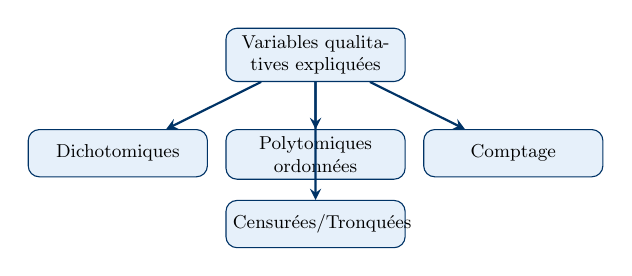
\begin{tikzpicture}[scale=0.75, every node/.style={transform shape},
            node distance=1.2cm,
            box/.style={rectangle, draw=darkblue, fill=lightblue, text width=2.8cm, align=center, minimum height=0.8cm, rounded corners, font=\small},
            arrow/.style={->, >=stealth, thick, darkblue}
        ]
        \node[box] (qual) {Variables qualitatives expliquées};
        \node[box, below left=0.8cm and 0.3cm of qual] (dicho) {Dichotomiques};
        \node[box, below=0.8cm of qual] (poly) {Polytomiques ordonnées};
        \node[box, below right=0.8cm and 0.3cm of qual] (count) {Comptage};
        \node[box, below=2cm of qual] (cens) {Censurées/Tronquées};
        
        \draw[arrow] (qual) -- (dicho);
        \draw[arrow] (qual) -- (poly);
        \draw[arrow] (qual) -- (count);
        \draw[arrow] (qual) -- (cens);
        \end{tikzpicture}
    \end{center}
\end{frame}

% --------------------------------------------
\subsection{Variables dichotomiques}

\begin{frame}{Définition et codage}
    \begin{definitionfr}[Variable dichotomique]
        Une variable dichotomique ne peut prendre que deux modalités exclusives l'une de l'autre (Oui/Non, Supérieur/Inférieur à un seuil, etc.).
        
        \vspace{0.2cm}
        
        Par convention, on code :
        \[
        y_i = \begin{cases}
            1 & \text{si l'événement se produit} \\
            0 & \text{sinon}
        \end{cases}
        \]
    \end{definitionfr}
    
    \begin{exemplefr}[Innovation]
        \[
        y_i = \begin{cases}
            1 & \text{si l'entreprise } i \text{ a innové} \\
            0 & \text{sinon}
        \end{cases}
        \]
    \end{exemplefr}
\end{frame}

\begin{frame}{Objectif économétrique}
    \begin{block}{Ce que l'on cherche à expliquer}
        Les déterminants de la \alert{probabilité} que l'événement se produise :
        \[
        \Prob(y_i = 1 \mid X_i) = ?
        \]
        On cherche les variables qui augmentent ou réduisent cette probabilité.
    \end{block}
    
    \vspace{0.3cm}
    
    \begin{block}{Approche par variable latente}
        On construit un \textbf{modèle latent} (inobservable) qui représente le critère de décision sous-jacent.
    \end{block}
\end{frame}

\begin{frame}{Le modèle latent}
    \begin{block}{Spécification}
        Soit $\pi_i^*$ une variable latente (inobservable) :
        \[
        \pi_i^* = X_i b + u_i, \quad i = 1, \ldots, N
        \]
    \end{block}
    
    \begin{exemplefr}[Innovation]
        $\pi_i^*$ représente l'espérance de profit associée à l'introduction d'une innovation, compte tenu d'un effet de remplacement des anciens produits.
    \end{exemplefr}
    
    \vspace{0.3cm}
    
    \begin{block}{Lien observé-latent}
        L'innovation n'est observée que si le gain anticipé dépasse un seuil $\pi_0$ :
        \[
        y_i = \begin{cases}
            1 & \text{si } \pi_i^* > \pi_0 \\
            0 & \text{si } \pi_i^* \leq \pi_0
        \end{cases}
        \]
    \end{block}
\end{frame}

\begin{frame}{Calcul de la probabilité}
    \begin{propositionfr}
        La probabilité d'observer $y_i = 1$ est :
        \[
        \Prob(y_i = 1) = \Prob(\pi_i^* > \pi_0) = \Prob(X_i b + u_i > \pi_0)
        \]
    \end{propositionfr}
    
    \vspace{0.3cm}
    
    \begin{block}{Forme fonctionnelle}
        La forme explicite dépend de l'hypothèse sur la distribution de $u_i$ :
        \begin{itemize}
            \item \textbf{Loi logistique} $\Rightarrow$ Modèle \alert{Logit}
            \item \textbf{Loi normale} $\Rightarrow$ Modèle \alert{Probit}
        \end{itemize}
    \end{block}
    
    \begin{remarquefr}
        D'autres distributions sont possibles ; des tests permettent de choisir la spécification appropriée.
    \end{remarquefr}
\end{frame}

\begin{frame}{Schéma récapitulatif}
    \begin{center}
        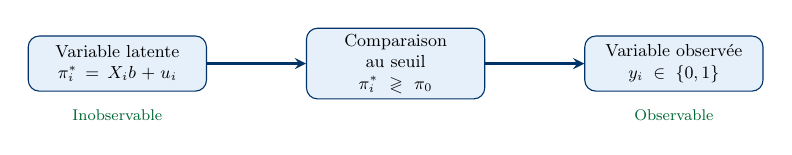
\begin{tikzpicture}[scale=0.7, every node/.style={transform shape},
            node distance=1.5cm,
            box/.style={rectangle, draw=darkblue, fill=lightblue, text width=3cm, align=center, minimum height=1cm, rounded corners, font=\small},
            arrow/.style={->, >=stealth, thick, darkblue}
        ]
        \node[box] (latent) {Variable latente\\$\pi_i^* = X_i b + u_i$};
        \node[box, right=1.8cm of latent] (seuil) {Comparaison au seuil\\$\pi_i^* \gtrless \pi_0$};
        \node[box, right=1.8cm of seuil] (obs) {Variable observée\\$y_i \in \{0, 1\}$};
        
        \draw[arrow] (latent) -- (seuil);
        \draw[arrow] (seuil) -- (obs);
        
        \node[below=0.2cm of latent, text=darkgreen, font=\footnotesize] {Inobservable};
        \node[below=0.2cm of obs, text=darkgreen, font=\footnotesize] {Observable};
        \end{tikzpicture}
    \end{center}
    
    \vspace{0.5cm}
    
    \begin{block}{Information utilisable}
        Seules les variables $(y_i, X_i)$ sont observables et utilisables pour l'estimation.
    \end{block}
\end{frame}

% --------------------------------------------
\subsection{Variables polytomiques ordonnées}

\begin{frame}{Définition}
    \begin{definitionfr}[Variable polytomique ordonnée]
        Variable qualitative à plus de deux modalités, ordonnées entre elles.
    \end{definitionfr}
    
    \begin{exemplefr}
        \begin{itemize}
            \item \textbf{Quantitative discrétisée} : Part des produits innovants dans le CA
            \begin{center}
                \small $[0\%-10\%]$, $]10\%-30\%]$, $]30\%-70\%]$, $]70\%-100\%]$
            \end{center}
            
            \item \textbf{Appréciation subjective} : Importance de la R\&D comme déterminant
            \begin{center}
                \small "Pas du tout", "Un peu", "Moyennement", "Beaucoup"
            \end{center}
        \end{itemize}
    \end{exemplefr}
    
    \begin{remarquefr}
        Dans les deux cas, les modalités traduisent un \alert{ordre} qui indique l'intensité de la variable.
    \end{remarquefr}
\end{frame}

\begin{frame}{Modèle latent}
    \begin{block}{Variable latente continue}
        Le modèle latent représente la "vraie valeur" de la variable :
        \[
        y_i^* = X_i b + u_i, \quad i = 1, \ldots, N
        \]
    \end{block}
    
    \begin{block}{Observation par intervalle}
        La variable observable prend $r$ modalités :
        \[
        y_i = \begin{cases}
            1 & \text{si } \alpha_0 < y_i^* \leq \alpha_1 \\
            2 & \text{si } \alpha_1 < y_i^* \leq \alpha_2 \\
            \vdots \\
            r & \text{si } \alpha_{r-1} < y_i^* \leq \alpha_r
        \end{cases}
        \]
        avec par convention $\alpha_0 = -\infty$ et $\alpha_r = +\infty$.
    \end{block}
\end{frame}

\begin{frame}{Représentation graphique}
    \begin{center}
        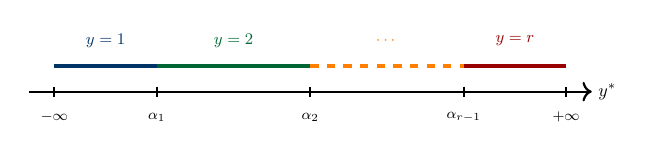
\begin{tikzpicture}[scale=0.65, every node/.style={transform shape}]
            % Axe
            \draw[thick, ->] (-0.5,0) -- (10.5,0) node[right] {$y^*$};
            
            % Seuils
            \foreach \x in {0, 2, 5, 8, 10} {
                \draw[thick] (\x,0.1) -- (\x,-0.1);
            }
            \node at (0,-0.5) {\footnotesize $-\infty$};
            \node at (2,-0.5) {\footnotesize $\alpha_1$};
            \node at (5,-0.5) {\footnotesize $\alpha_2$};
            \node at (8,-0.5) {\footnotesize $\alpha_{r-1}$};
            \node at (10,-0.5) {\footnotesize $+\infty$};
            
            % Modalités
            \draw[darkblue, very thick] (0,0.5) -- (2,0.5);
            \node[darkblue] at (1,1) {\small $y=1$};
            
            \draw[darkgreen, very thick] (2,0.5) -- (5,0.5);
            \node[darkgreen] at (3.5,1) {\small $y=2$};
            
            \draw[orange, very thick, dashed] (5,0.5) -- (8,0.5);
            \node[orange] at (6.5,1) {\small $\cdots$};
            
            \draw[darkred, very thick] (8,0.5) -- (10,0.5);
            \node[darkred] at (9,1) {\small $y=r$};
        \end{tikzpicture}
    \end{center}
    
    \vspace{0.3cm}
    
    \begin{block}{Seuils}
        \begin{itemize}
            \item \textbf{Seuils connus} : cas des variables quantitatives discrétisées
            \item \textbf{Seuils inconnus} : cas des appréciations subjectives (à estimer)
        \end{itemize}
    \end{block}
\end{frame}

\begin{frame}{Probabilités des modalités}
    \begin{propositionfr}
        La probabilité d'observer la modalité $j$ est :
        \begin{align*}
            \Prob(y_i = j) &= \Prob(\alpha_{j-1} < y_i^* \leq \alpha_j) \\
            &= \Prob(y_i^* \leq \alpha_j) - \Prob(y_i^* \leq \alpha_{j-1})
        \end{align*}
        pour $j = 1, \ldots, r$.
    \end{propositionfr}
    
    \vspace{0.3cm}
    
    \begin{block}{Modèle Probit ordonné}
        Si $u_i \sim \mathcal{N}(0, \sigma^2)$ :
        \[
        \Prob(y_i = j) = \Phi\left(\frac{\alpha_j - X_i b}{\sigma}\right) - \Phi\left(\frac{\alpha_{j-1} - X_i b}{\sigma}\right)
        \]
        où $\Phi$ est la fonction de répartition de la loi normale centrée réduite.
    \end{block}
\end{frame}

% --------------------------------------------
\subsection{Variables de comptage}

\begin{frame}{Caractéristiques}
    \begin{definitionfr}[Variable de comptage]
        Variable prenant ses valeurs dans $\N = \{0, 1, 2, \ldots\}$, représentant le nombre d'occurrences d'un événement.
    \end{definitionfr}
    
    \begin{exemplefr}[Brevets]
        Le nombre de brevets déposés par une entreprise sur une année :
        \begin{itemize}
            \item Valeurs entières positives ou nulles
            \item Événements relativement rares
            \item Beaucoup d'entreprises à 0 brevet
        \end{itemize}
    \end{exemplefr}
    
    \begin{remarquefr}
        Ce n'est pas une variable quantitative classique : elle ne peut pas prendre de valeurs négatives et a une nature discrète.
    \end{remarquefr}
\end{frame}

\begin{frame}{Modélisation}
    \begin{block}{Espérance conditionnelle}
        L'espérance étant toujours strictement positive, on utilise une forme exponentielle :
        \[
        \E(y_i \mid X_i, b) = \exp(X_i b + u_i) > 0
        \]
    \end{block}
    
    \vspace{0.3cm}
    
    \begin{block}{Loi de Poisson}
        On suppose que $y_i$ suit une \alert{loi de Poisson} de paramètre $\lambda_i = \exp(X_i b)$ :
        \[
        \Prob(y_i = k) = \frac{\exp(-\lambda_i) \lambda_i^k}{k!}, \quad k = 0, 1, 2, \ldots
        \]
    \end{block}
\end{frame}

\begin{frame}{Sources d'aléa}
    \begin{alertblock}{Double source d'aléa}
        \begin{enumerate}
            \item \textbf{Erreur sur la moyenne} : $\exp(u_i)$ (incertitude sur l'espérance)
            \item \textbf{Tirage de Poisson} : aléa intrinsèque du processus de comptage
        \end{enumerate}
    \end{alertblock}
    
    \vspace{0.3cm}
    
    \begin{block}{Distinction}
        \begin{itemize}
            \item \textbf{Modèle de Poisson homogène} : $\Var[\exp(u_i)] = 0$ (pas d'hétérogénéité inobservée)
            \item \textbf{Modèle de Poisson hétérogène} : $\Var[\exp(u_i)] > 0$ (hétérogénéité présente)
        \end{itemize}
    \end{block}
    
    \begin{remarquefr}
        Le modèle de Poisson homogène correspond à une loi de durée exponentielle pour le temps entre événements.
    \end{remarquefr}
\end{frame}

% --------------------------------------------
\subsection{Variables censurées ou tronquées}

\begin{frame}{Définition}
    \begin{definitionfr}[Variable censurée/tronquée]
        Variable dont on n'observe la réalisation que pour certains individus, en raison :
        \begin{itemize}
            \item Du processus de collecte des données (censure exogène)
            \item D'une décision prise par les individus (censure endogène)
        \end{itemize}
    \end{definitionfr}
    
    \vspace{0.3cm}
    
    \begin{exemplefr}[R\&D]
        Une entreprise doit décider :
        \begin{enumerate}
            \item Si elle investit en R\&D (décision de participation)
            \item Combien elle investit (montant, observé seulement si participation)
        \end{enumerate}
        Ces deux décisions sont étroitement reliées.
    \end{exemplefr}
\end{frame}

\begin{frame}{Le modèle Tobit généralisé}
    \begin{block}{Équation de sélection}
        Le critère de décision est modélisé par une variable latente $\pi_i^*$ :
        \[
        \pi_i^* = X_{1i} b_1 + u_{1i}, \quad i = 1, \ldots, N
        \]
        La décision de participer est :
        \[
        y_i = \begin{cases}
            1 & \text{si } \pi_i^* \geq 0 \\
            0 & \text{si } \pi_i^* < 0
        \end{cases}
        \]
    \end{block}
    
    \begin{block}{Équation de résultat}
        Le montant investi est déterminé par :
        \[
        r_i^* = X_{2i} b_2 + u_{2i}, \quad i = 1, \ldots, N
        \]
    \end{block}
\end{frame}

\begin{frame}{Observation et corrélation}
    \begin{block}{Variable observable}
        Le montant n'est observé que si l'entreprise participe :
        \[
        r_i = \begin{cases}
            r_i^* & \text{si } \pi_i^* \geq 0 \\
            \text{manquant} & \text{si } \pi_i^* < 0
        \end{cases}
        \]
    \end{block}
    
    \vspace{0.3cm}
    
    \begin{alertblock}{Corrélation des équations}
        Les deux variables latentes $\pi_i^*$ et $r_i^*$ sont généralement \alert{corrélées} :
        \begin{itemize}
            \item Le montant optimal $r^*$ est obtenu en maximisant le profit $\pi^*$
            \item Les deux décisions sont déterminées simultanément
        \end{itemize}
        Cette corrélation génère un \textbf{biais de sélection} si on l'ignore.
    \end{alertblock}
\end{frame}

\begin{frame}{Modèle de Heckman}
    \begin{theoremefr}[Modèle Tobit généralisé]
        Si les perturbations suivent une loi normale bivariée :
        \[
        \begin{pmatrix} u_{1i} \\ u_{2i} \end{pmatrix} \sim \mathcal{N}\left( \begin{pmatrix} 0 \\ 0 \end{pmatrix}, \begin{pmatrix} \sigma_1^2 & \rho\sigma_1\sigma_2 \\ \rho\sigma_1\sigma_2 & \sigma_2^2 \end{pmatrix} \right)
        \]
        on obtient le \alert{modèle Tobit généralisé de Heckman}.
    \end{theoremefr}
    
    \vspace{0.3cm}
    
    \begin{block}{Paramètre clé}
        Le coefficient de corrélation $\rho$ :
        \begin{itemize}
            \item Si $\rho = 0$ : pas de biais de sélection, on peut estimer séparément
            \item Si $\rho \neq 0$ : biais de sélection, il faut corriger (procédure de Heckman)
        \end{itemize}
    \end{block}
\end{frame}

\begin{frame}{Schéma du processus}
    \begin{center}
        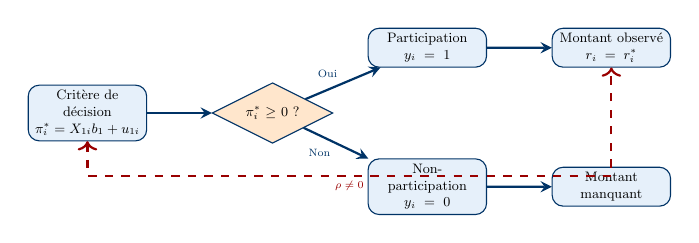
\begin{tikzpicture}[scale=0.55, every node/.style={transform shape},
            node distance=1cm,
            box/.style={rectangle, draw=darkblue, fill=lightblue, text width=2.5cm, align=center, minimum height=0.8cm, rounded corners, font=\small},
            decision/.style={diamond, draw=darkblue, fill=orange!20, text width=1.5cm, align=center, aspect=2, font=\small},
            arrow/.style={->, >=stealth, thick, darkblue}
        ]
        
        \node[box] (latent1) {Critère de décision\\$\pi_i^* = X_{1i} b_1 + u_{1i}$};
        \node[decision, right=1.5cm of latent1] (dec) {$\pi_i^* \geq 0$ ?};
        \node[box, above right=0.7cm and 1.5cm of dec] (oui) {Participation\\$y_i = 1$};
        \node[box, below right=0.7cm and 1.5cm of dec] (non) {Non-participation\\$y_i = 0$};
        \node[box, right=1.5cm of oui] (result) {Montant observé\\$r_i = r_i^*$};
        \node[box, right=1.5cm of non] (manq) {Montant manquant};
        
        \draw[arrow] (latent1) -- (dec);
        \draw[arrow] (dec) -- node[above left, font=\scriptsize] {Oui} (oui);
        \draw[arrow] (dec) -- node[below left, font=\scriptsize] {Non} (non);
        \draw[arrow] (oui) -- (result);
        \draw[arrow] (non) -- (manq);
        
        % Corrélation
        \draw[darkred, dashed, thick, <->] (latent1.south) -- ++(0,-0.8) -| node[pos=0.25, below, font=\scriptsize] {$\rho \neq 0$} (result.south);
        \end{tikzpicture}
    \end{center}
\end{frame}

% ============================================
% RÉCAPITULATIF
% ============================================

{
\setbeamercolor{background canvas}{bg=darkred}
\setbeamercolor{normal text}{fg=white}
\usebeamercolor[fg]{normal text}
\begin{frame}[plain]
    \vfill
    \begin{center}
        {\Huge\bfseries SYNTHÈSE}
        
        \vspace{1cm}
        
        {\LARGE Récapitulatif des deux parties}
        
        \vspace{1.5cm}
        
        
\begin{tikzpicture}
            \node[rectangle, fill=white, rounded corners, minimum width=3.5cm, minimum height=0.8cm, text=darkblue] at (-3,0) {\textbf{Partie I : Explicatives}};
            \node[rectangle, fill=white, rounded corners, minimum width=3.5cm, minimum height=0.8cm, text=darkgreen] at (3,0) {\textbf{Partie II : Expliquées}};
        \end{tikzpicture}
    \end{center}
    \vfill
\end{frame}
}

\section{Récapitulatif}

\begin{frame}{Synthèse — \textcolor{darkblue}{Partie I : Variables explicatives}}
    \begin{center}
        \small
        \begin{tabular}{lll}
            \toprule
            \textbf{Modèle} & \textbf{Interprétation de $b_j$} & \textbf{Remarque} \\
            \midrule
            Sans constante & $\E(y \mid \text{groupe } j)$ & Moyenne du groupe \\
            Avec constante & $\E(y \mid j) - \E(y \mid k)$ & Écart à la référence $k$ \\
            Avec $X$ & Idem, à $X$ fixé & Effet contrôlé \\
            Avec interactions & Effet hétérogène & Centrer $X$ simplifie \\
            \bottomrule
        \end{tabular}
    \end{center}
    
    \vspace{0.3cm}
    
    \begin{alertblock}{Points clés — Variables qualitatives \textbf{à droite}}
        \begin{itemize}
            \item Toujours indiquer la modalité de référence
            \item Le test de Fisher teste l'égalité des moyennes entre groupes
            \item Centrer les variables avant les produits croisés facilite l'interprétation
        \end{itemize}
    \end{alertblock}
\end{frame}

\begin{frame}{Synthèse — \textcolor{darkgreen}{Partie II : Variables expliquées}}
    \begin{center}
        \small
        \begin{tabular}{llll}
            \toprule
            \textbf{Type} & \textbf{Valeurs} & \textbf{Modèle} & \textbf{Estimation} \\
            \midrule
            Dichotomique & $\{0, 1\}$ & Logit/Probit & MV \\
            Polytomique ordonnée & $\{1, \ldots, r\}$ & Probit ordonné & MV \\
            Comptage & $\N$ & Poisson & MV/PMV \\
            Censurée & Continue + sélection & Tobit/Heckman & MV \\
            \bottomrule
        \end{tabular}
    \end{center}
    
    \vspace{0.3cm}
    
    \begin{exampleblock}{Principe commun — Variables qualitatives \textbf{à gauche}}
        \begin{enumerate}
            \item Spécifier un \textbf{modèle latent} pour le phénomène sous-jacent
            \item Définir le \textbf{lien} entre variable latente et variable observée
            \item \textbf{Estimer} par maximum de vraisemblance
        \end{enumerate}
    \end{exampleblock}
\end{frame}

\begin{frame}{Pour aller plus loin}
    \begin{block}{Chapitres suivants}
        \begin{itemize}
            \item \textbf{Chapitre 2} : Maximum de vraisemblance (théorie et propriétés)
            \item \textbf{Chapitre 3} : Modèles Logit et Probit en détail
            \item \textbf{Chapitre 4} : Variables polytomiques
            \item \textbf{Chapitres 5} : Extensions
        \end{itemize}
    \end{block}
    
    \vspace{0.3cm}
    
    \begin{block}{Références}
      \begin{itemize}
        \item
            \item Gouriéroux, C. (1989). \textit{Économétrie des variables qualitatives}
            \item Maddala, G.S. (1983). \textit{Limited-Dependent and Qualitative Variables in Econometrics}
        \end{itemize}
    \end{block}
\end{frame}

\end{document}
